%!TEX root = ../terrainbook.tex
% chktex-file 46

% \setchapterpreamble[u]{\margintoc \marginnote{\faYoutube\ https://3d.bk.tudelft.nl}}
% TODO : youtube link?
\setchapterpreamble[u]{\margintoc}
% \setchapterpreamble[u]{\marginnote{\faYoutube\ https://3d.bk.tudelft.nl}}

\chapter{Handling massive terrains}
\label{chap:massive}


\graphicspath{{massive/}}


In this chapter we discuss three methods to deal with massive terrains (or input datasets).

%

``Massive'' is a vague and undefined term in GIS, and it is continuously changing: 10 years ago a point cloud dataset containing 5 million points was considered massive, while in 2018 it is not.
There are some massive datasets even in small areas, \eg\ a Lidar one of Dublin\sidenote{\url{https://bit.ly/32GXiFq}}, containing around 1.4 billion points with a density of 300pts/m$^2$, which was collected with airborne laser scanners.
The lidar dataset of the Netherlands, AHN\sidenote{\emph{Actueel Hoogtebestand Nederland} (in Dutch): \url{http://www.ahn.nl}}, has about 10pts/m$^2$ covering the whole country, thus comprising more than 700 billion points which can be freely downloaded.
% TODO : other massive dataset examples? SRTM? Rotterdam?

%

For the purpose of this course, we define as ``massive'' a dataset that does not fit into the main memory of a standard computer, which is usually around 16GB\@.
This definition makes practical sense because working with data outside of the main memory of a computer is substantially slower (about 2 orders of magnitude for solid state drives and 5 for hard drives), causing many standard data processing algorithms to become impractical with massive datasets.
Keep in mind that not only the ($xyz$) coordinates of the points of a point cloud need to be stored, but also often attributes for each point (LAS has several standard ones).
Also, in the case of TINs, the geometry of the triangles---and potentially the topological relationships between them---need to be explicitly stored.

%

What is ironic is that while datasets like AHN3 are being collected in several countries, in practice they are seldom used since the tools that practitioners have, and are used to, usually cannot handle such massive datasets. 
Indeed, the traditional GISs and terrain modelling tools are limited by the main memory of computers: if a dataset is bigger then operations will be very slow, and will most likely not finish.



%%%%%%%%%%%%%%%%%%%%
%
\section{Raster Pyramids}%
\index{raster pyramid}

Raster pyramids are a well-known, standardised, and widely used mechanism to deal with large grids.
They are also used for images (and called `tiled pyramidal images' or `overview images') and many software support them since they optimise visualisation and thus the speed of a software dealing with large images.

As shown in \reffig{fig:pyramids}, 
\begin{figure}
  \centering
  \begin{subfigure}[b]{0.65\linewidth}
    \centering
    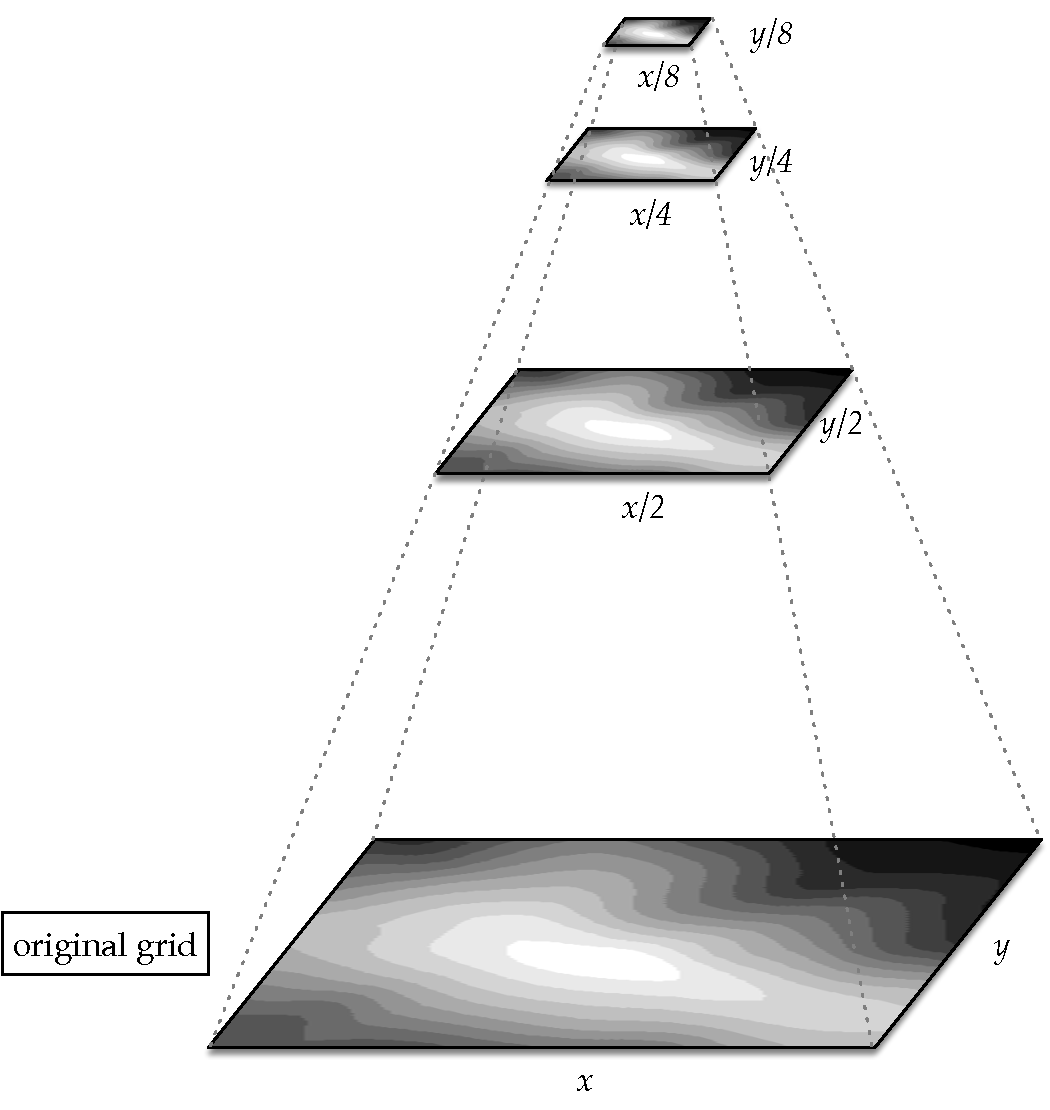
\includegraphics[width=\textwidth]{figs/pyramids.pdf}
    \caption{}
  \end{subfigure}
  \qquad%
  \begin{subfigure}[b]{0.2\linewidth}
    \centering
    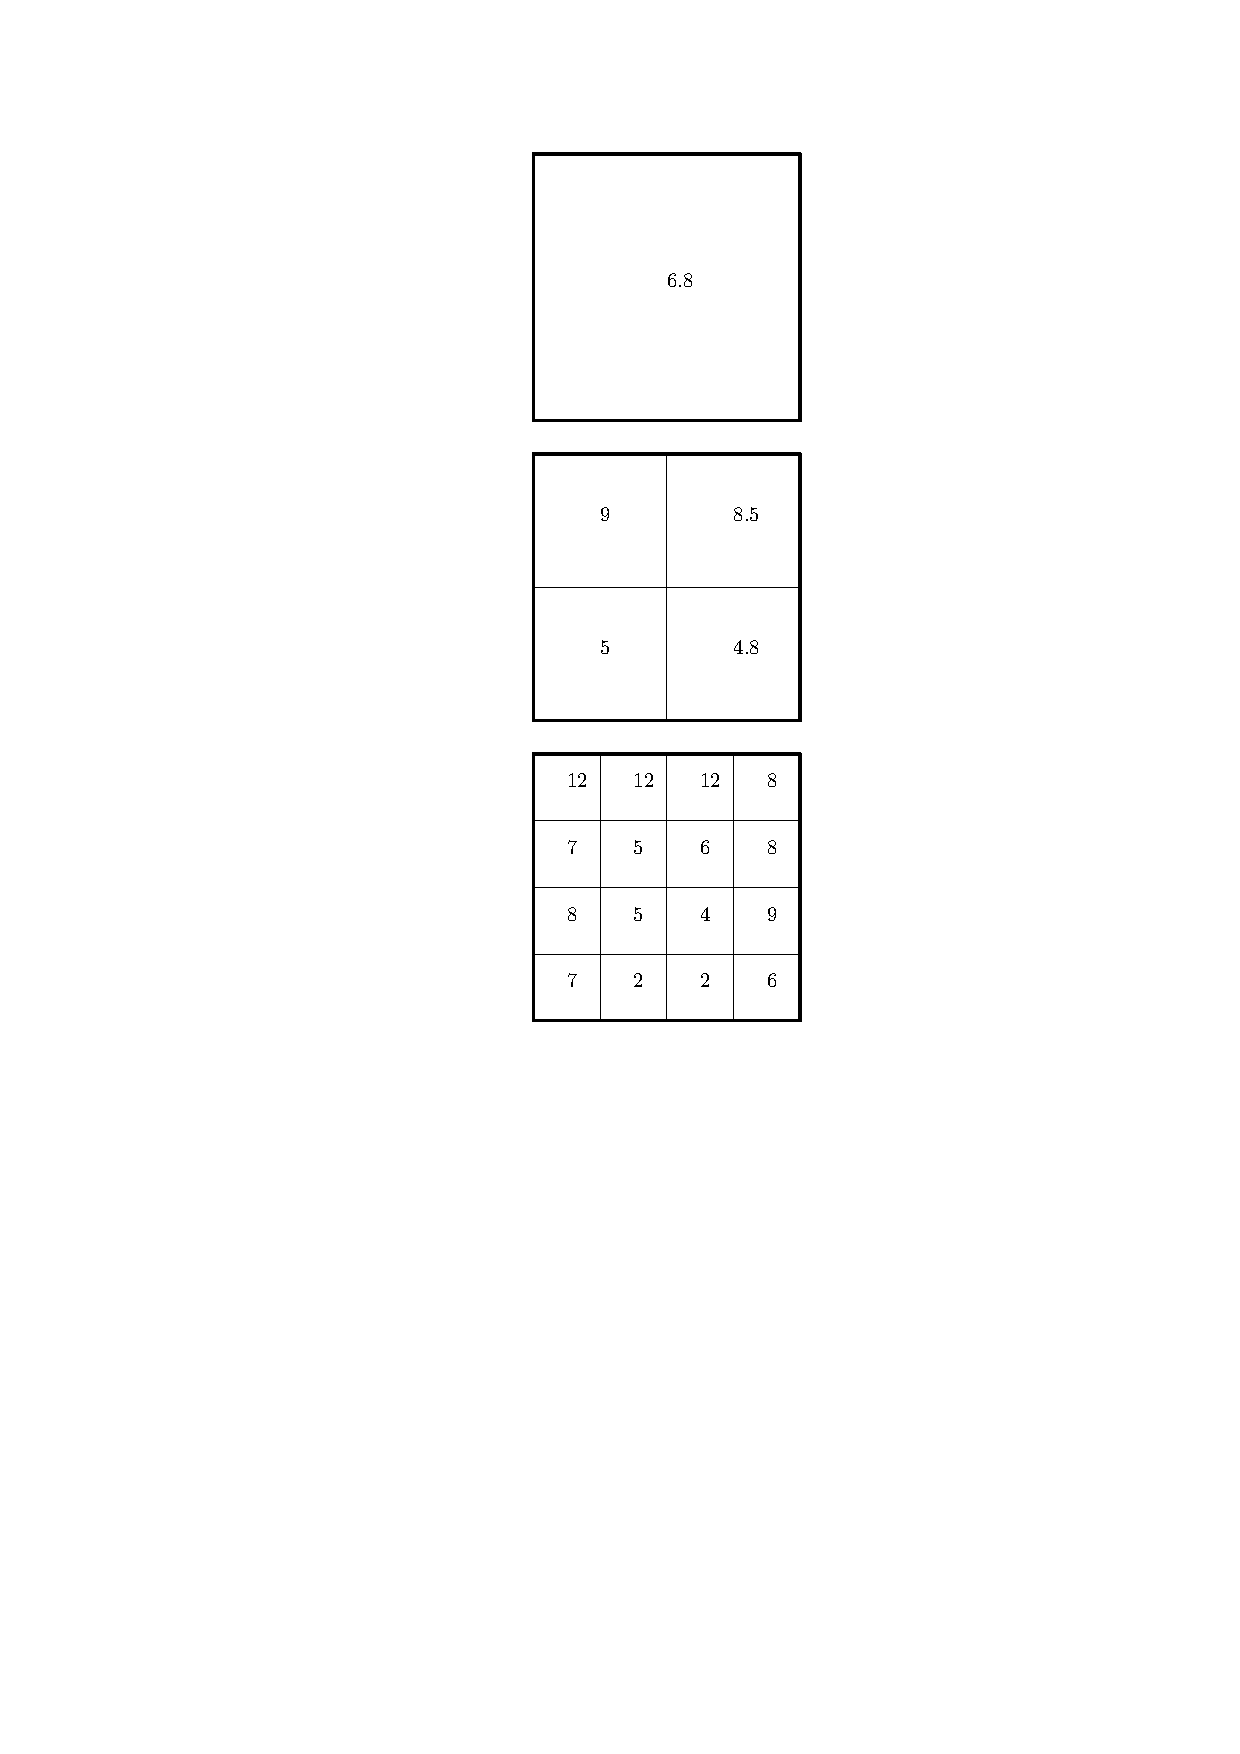
\includegraphics[width=\textwidth]{figs/pyramids2.pdf}
    \caption{}
  \end{subfigure}
\caption{\textbf{(a)} The pyramid for a given raster file. \textbf{(b)} One $4\times4$ raster downsampled twice with average-method.}%
\labfig{fig:pyramids}
\end{figure}
a pyramid means creating recursively copies at lower-resolutions of an original raster (having $x$ columns and $y$ rows), the first copy having a size ($\frac{x}{2}$, $\frac{y}{2}$), the second ($\frac{x}{4}$, $\frac{y}{4}$), and so on (the number of images is arbitrary and defined by the user).
Notice that the extra storage will be maximum $\frac{1}{3}$ of the original raster: the first pyramid is $\frac{1}{4}$, the second $\frac{1}{16}$, the third $\frac{1}{64}$, etc.

Each lower-resolution copy of the raster is obtained with \emph{downsampling}.
\index{downsampling}\marginnote{downsampling}
The most common method is based on averaging the 4 pixels that are merged into one (as shown in \reffig{fig:pyramids}b), but other methods are possible such as nearest neighbour (interpolation method as seen in \refchap{chap:interpol}).


\begin{kaobox-practice}[frametitle=\faCog\ How does it work in practice?]
  \textbf{gdaladdo.} 
  For certain formats, \eg\ GeoTIFF, the lower-resolutions rasters can be stored directly in the same file as the original raster, and this is standardised.
  For other formats in GIS, \eg\ the ASCII format `.asc', the pyramids are stored in an auxiliary file with the extension `.ovr', which is actually in TIFF format.

  The GDAL utility \texttt{gdaladdo} (\url{https://www.gdal.org/gdaladdo.html}) allows us to create automatically the pyramids for a few formats.
  The downsampling method can be chosen.
  % In QGIS, one can call \texttt{gdaladdo}, or there is also a built-in mechanism, as can be seen in \reffig{fig:qgis}
\end{kaobox-practice}

% \begin{marginfigure}
%   \centering
%   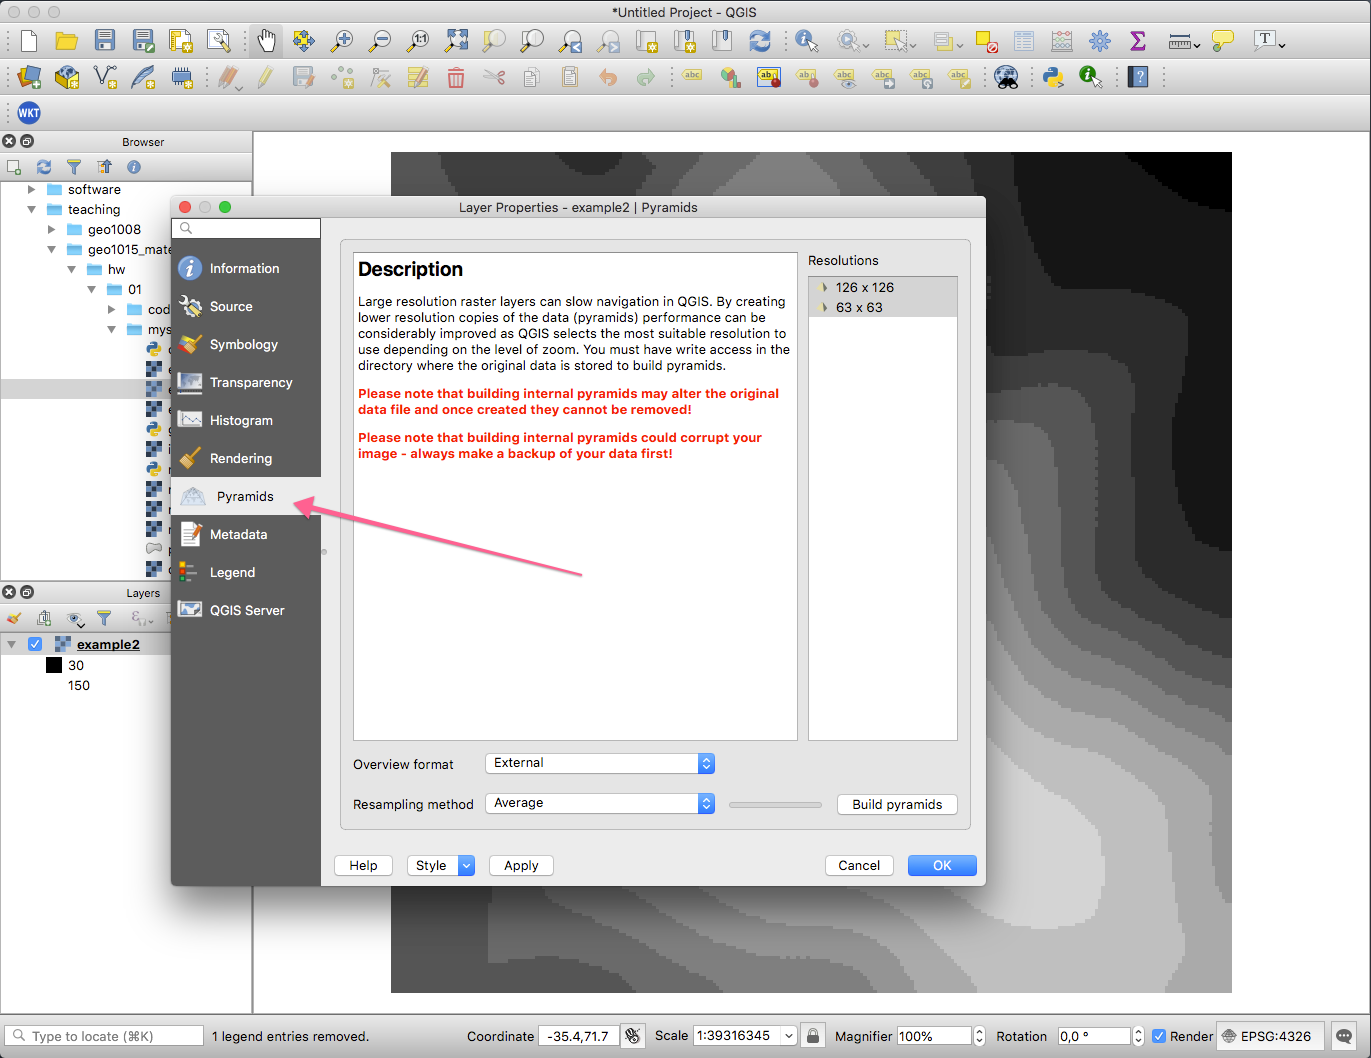
\includegraphics[width=\linewidth]{figs/qgis}
%   \caption{QGIS has the option to create the pyramids automatically.}%
% \labfig{fig:qgis}
% \end{marginfigure}



%%%%%%%%%%%%%%%%%%%%
%
\section[3D kd-tree]{Indexing points in 3D space with the kd-tree}%
\label{sec:kdtree}\index{kd-tree}

A $k$-dimensional tree, $k$d-tree in short, is a data structure to organise points in a $k$-dimensional space; it also partitions the space into regions.
In the context of terrains, $k$ is in most cases either 2 or 3.
Notice that in practice we would never say a ``2d-tree'' or a ``3d-tree'': we call them ``$k$d-tree of dimension 2 (or 3)''.

%

As shown in \reffig{fig:kdtree},
\begin{marginfigure}
  \centering
  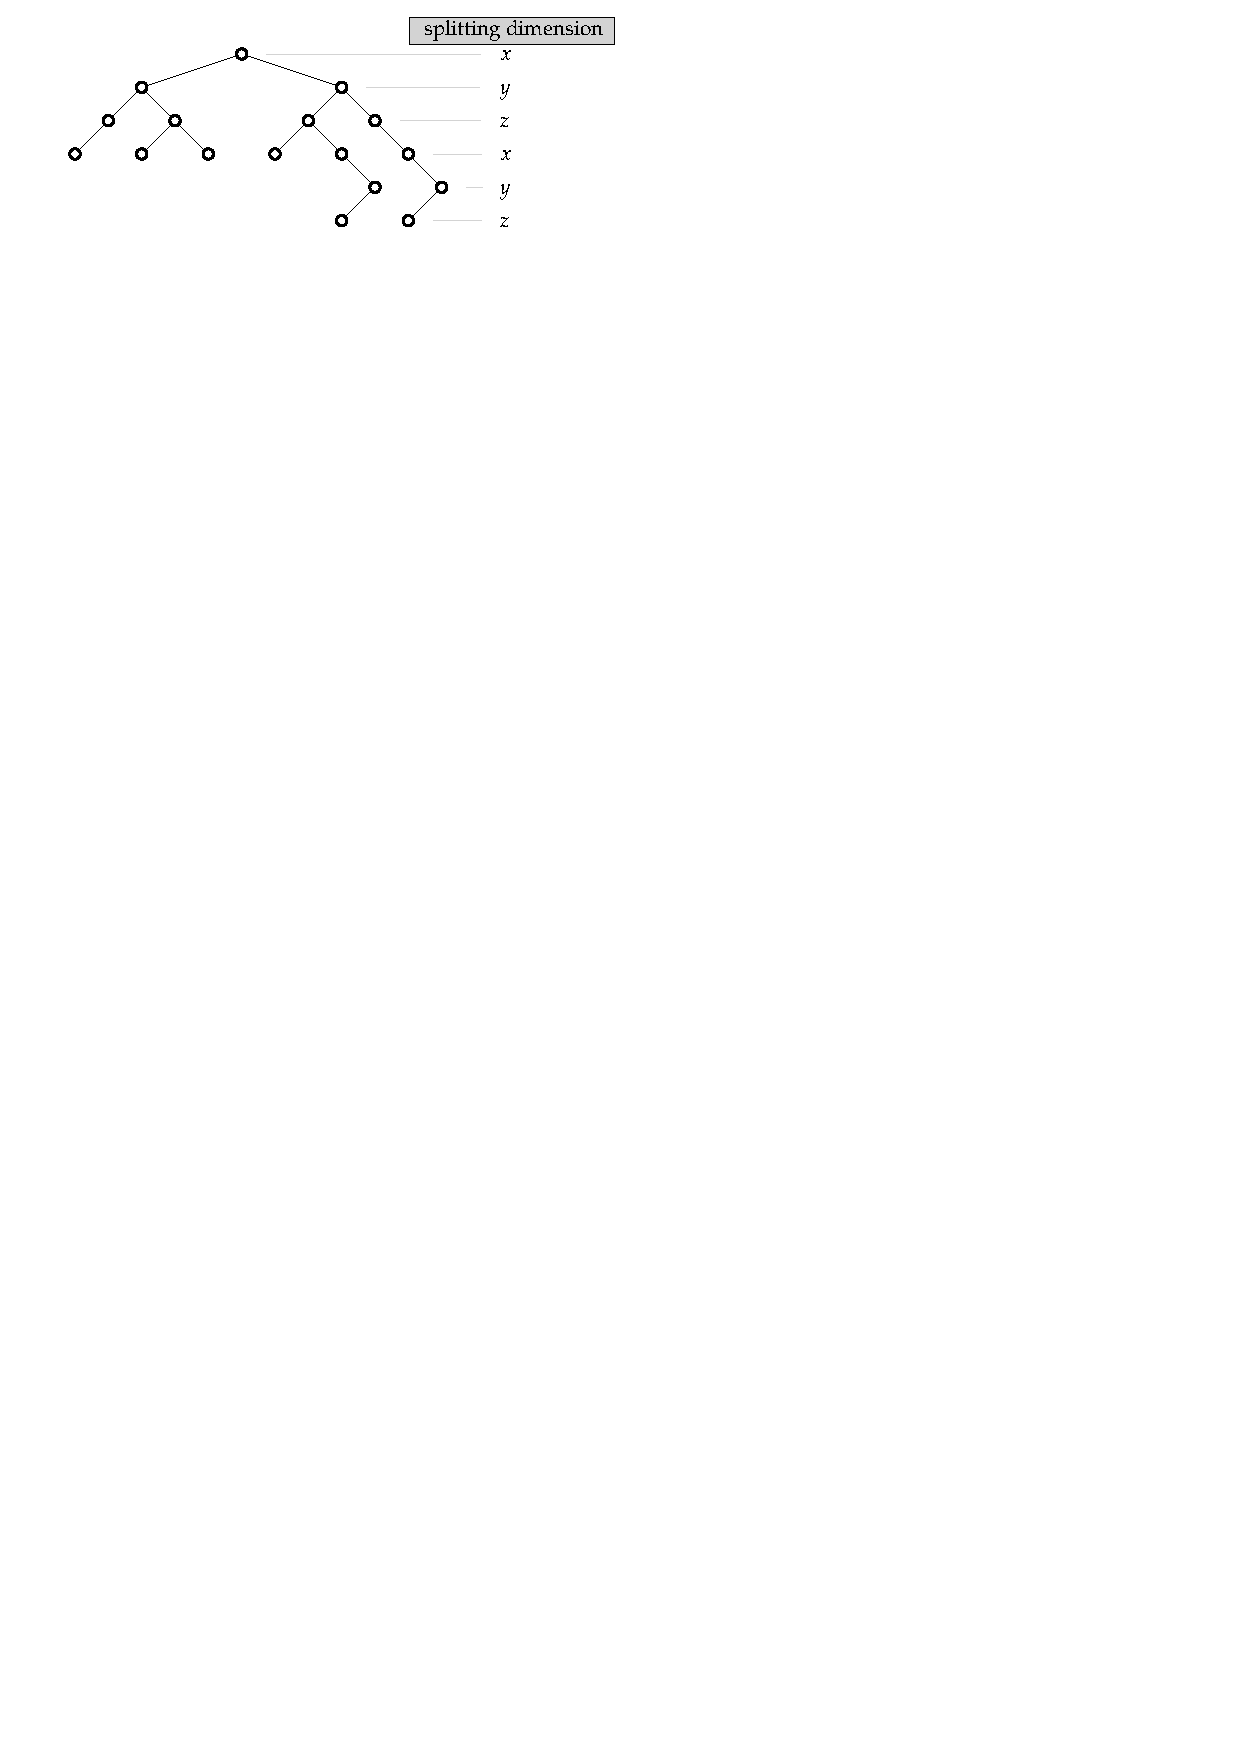
\includegraphics[width=\linewidth]{figs/kdtree}
  \caption{Example of $k$d-tree in 3D, with the dimensions used at each level.}%
\labfig{fig:kdtree}
\end{marginfigure} 
a $k$d-tree is a binary tree (thus each node has a maximum of 2 children, if any), and the main idea is that each level of the tree compares against one specific dimension.
We `cycle through' the dimensions as we walk down the levels of the tree.

%

Let $S$ be a set of points in $\mathbb{R}^k$, and let $\kappa$ be the $k$d-tree of dimension $k$ of $S$.
Each point $p_i$ in $S$ is a node of $\kappa$.
A node implies a hyperplane that divides the space into 2 halfspaces according to one dimension; the hyperplane is perpendicular to the dimension of the node (which is linked to the level in the tree).
Points with a lower coordinate value than the node along that dimension (corresponding to `left' or `under' the hyperplane) are put into the left subtree of the node, and the other ones into the right subtree.

Consider the $k$d-tree in 2D in \reffig{fig:kdtree2}.
\begin{figure}[tbp]
  \centering
  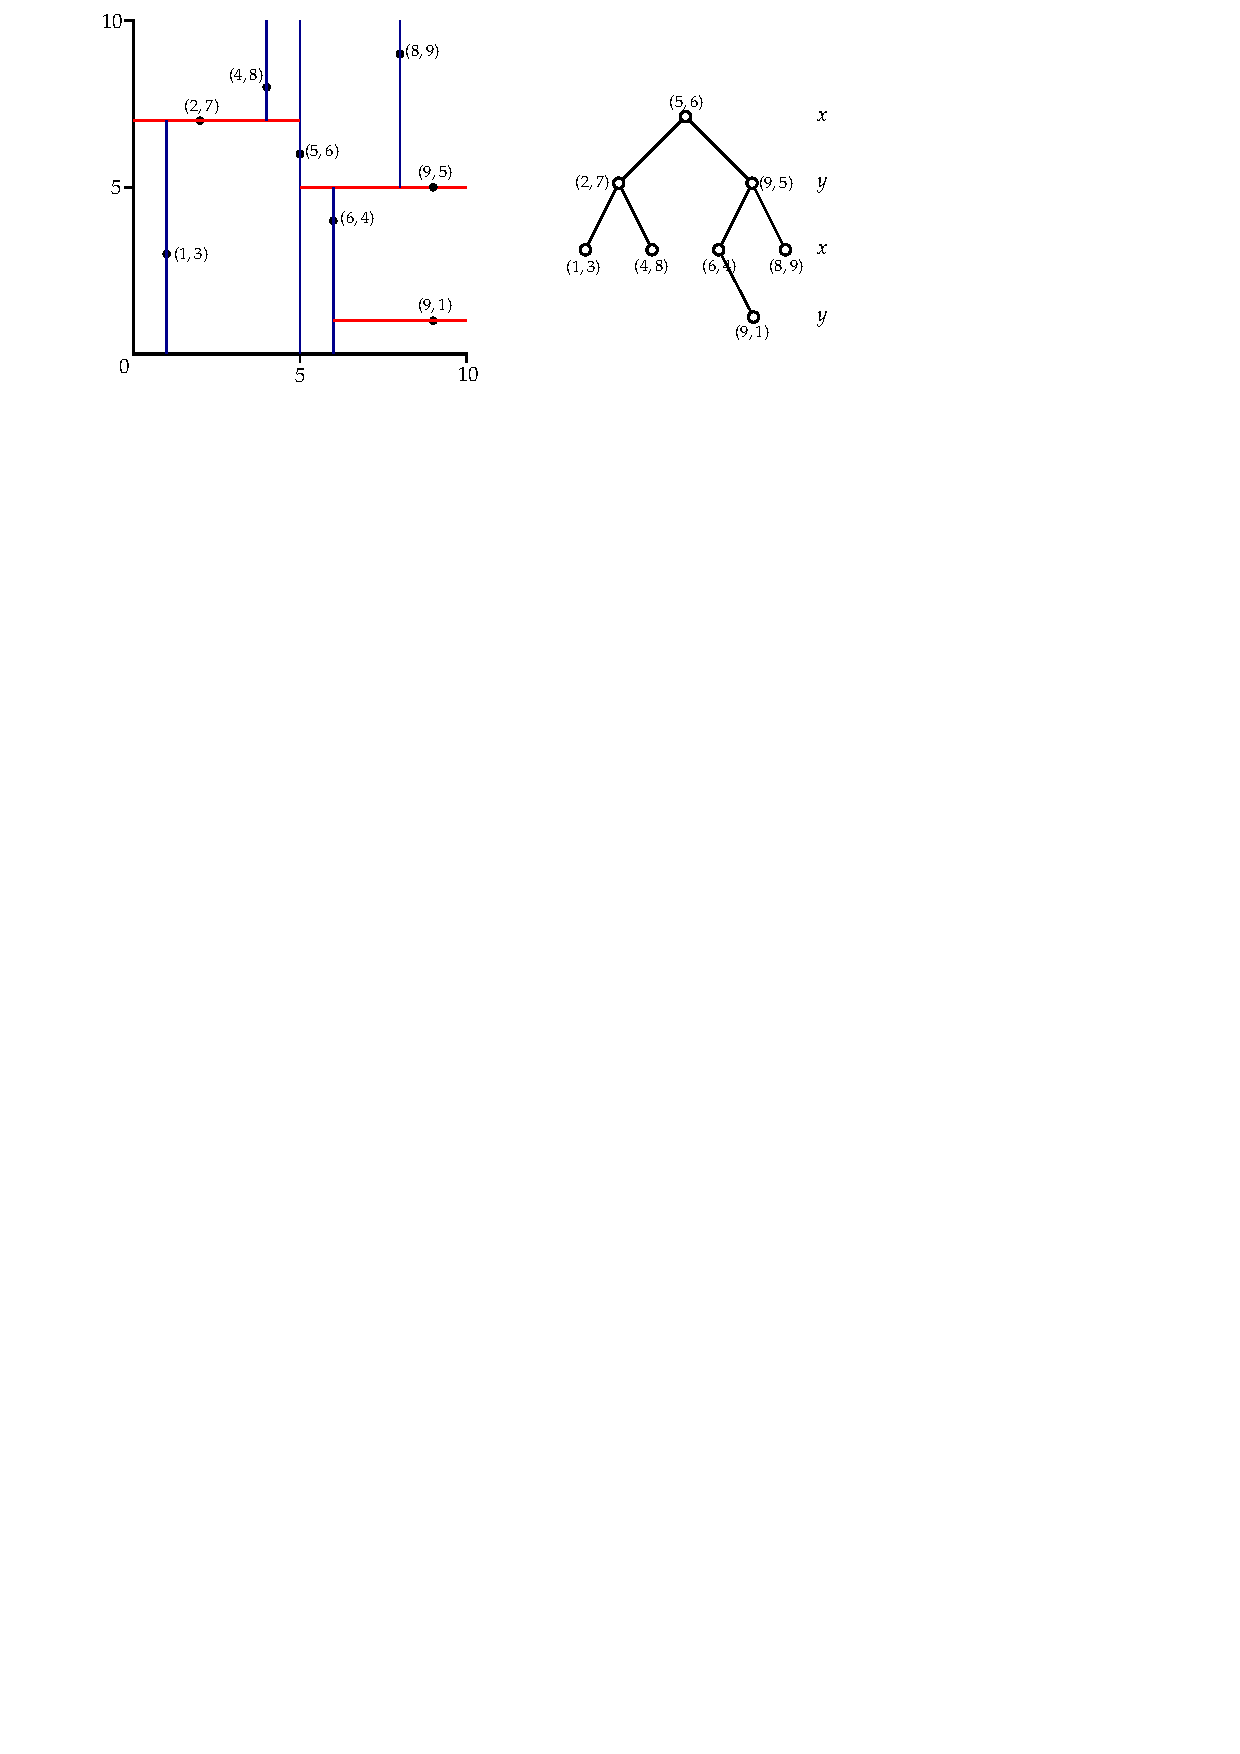
\includegraphics[width=0.9\linewidth]{figs/kdtree2}
  \caption{Example of $k$d-tree for 8 points in the $\mathbb{R}^2$.}%
\labfig{fig:kdtree2}
\end{figure}
The first dimension splits the data into 2 halfplanes along the line $x=5$, then each of these halfplanes is independently split according to the $y$ dimension (with the lines $y=7$ and $y=5$), then the 4 regions are split according to the $x$ dimension, and so on recursively.

%%%
\paragraph{Construction of a kd-tree.}
In theory, any point could be used to divide the space according to each dimension, and that would yield a valid $k$d-tree.
However, selecting the \emph{median} point creates a \emph{balanced} binary tree,%
\marginnote{binary tree} 
which is desirable because it will improve searching and visiting the tree (see below).
The tree in \reffig{fig:kdtree2} is balanced, but if for instance ($1,3$) had been selected as the root, then there would be no children on the left, and all of them would be on the right.

The median point is the one whose value for the splitting dimension is the median of all the points involved in the operation.
This implies that to construct the $k$d-tree of a set $S$ of $n$ points, as a first step $n$ values need to be sorted, which is a rather slow operation.
In practice, most software libraries will not sort $n$ values, but rather sample randomly a subset of them (say 1\%), and then use the median of this subset as the splitting node in the graph.
While this does not guarantee a balanced tree, in practice the tree should be close to balanced.

The tree is built incrementally, \ie\ points are added in the tree one after the other, and after each insertion the tree is updated.
Each insertion is simple: traverse the tree starting from the root, go left or right depending on the splitting dimension value, and insert the new point as a new leaf in the tree.
\reffig{fig:kdtree_insert}
\begin{figure}[tbp]
  \centering
  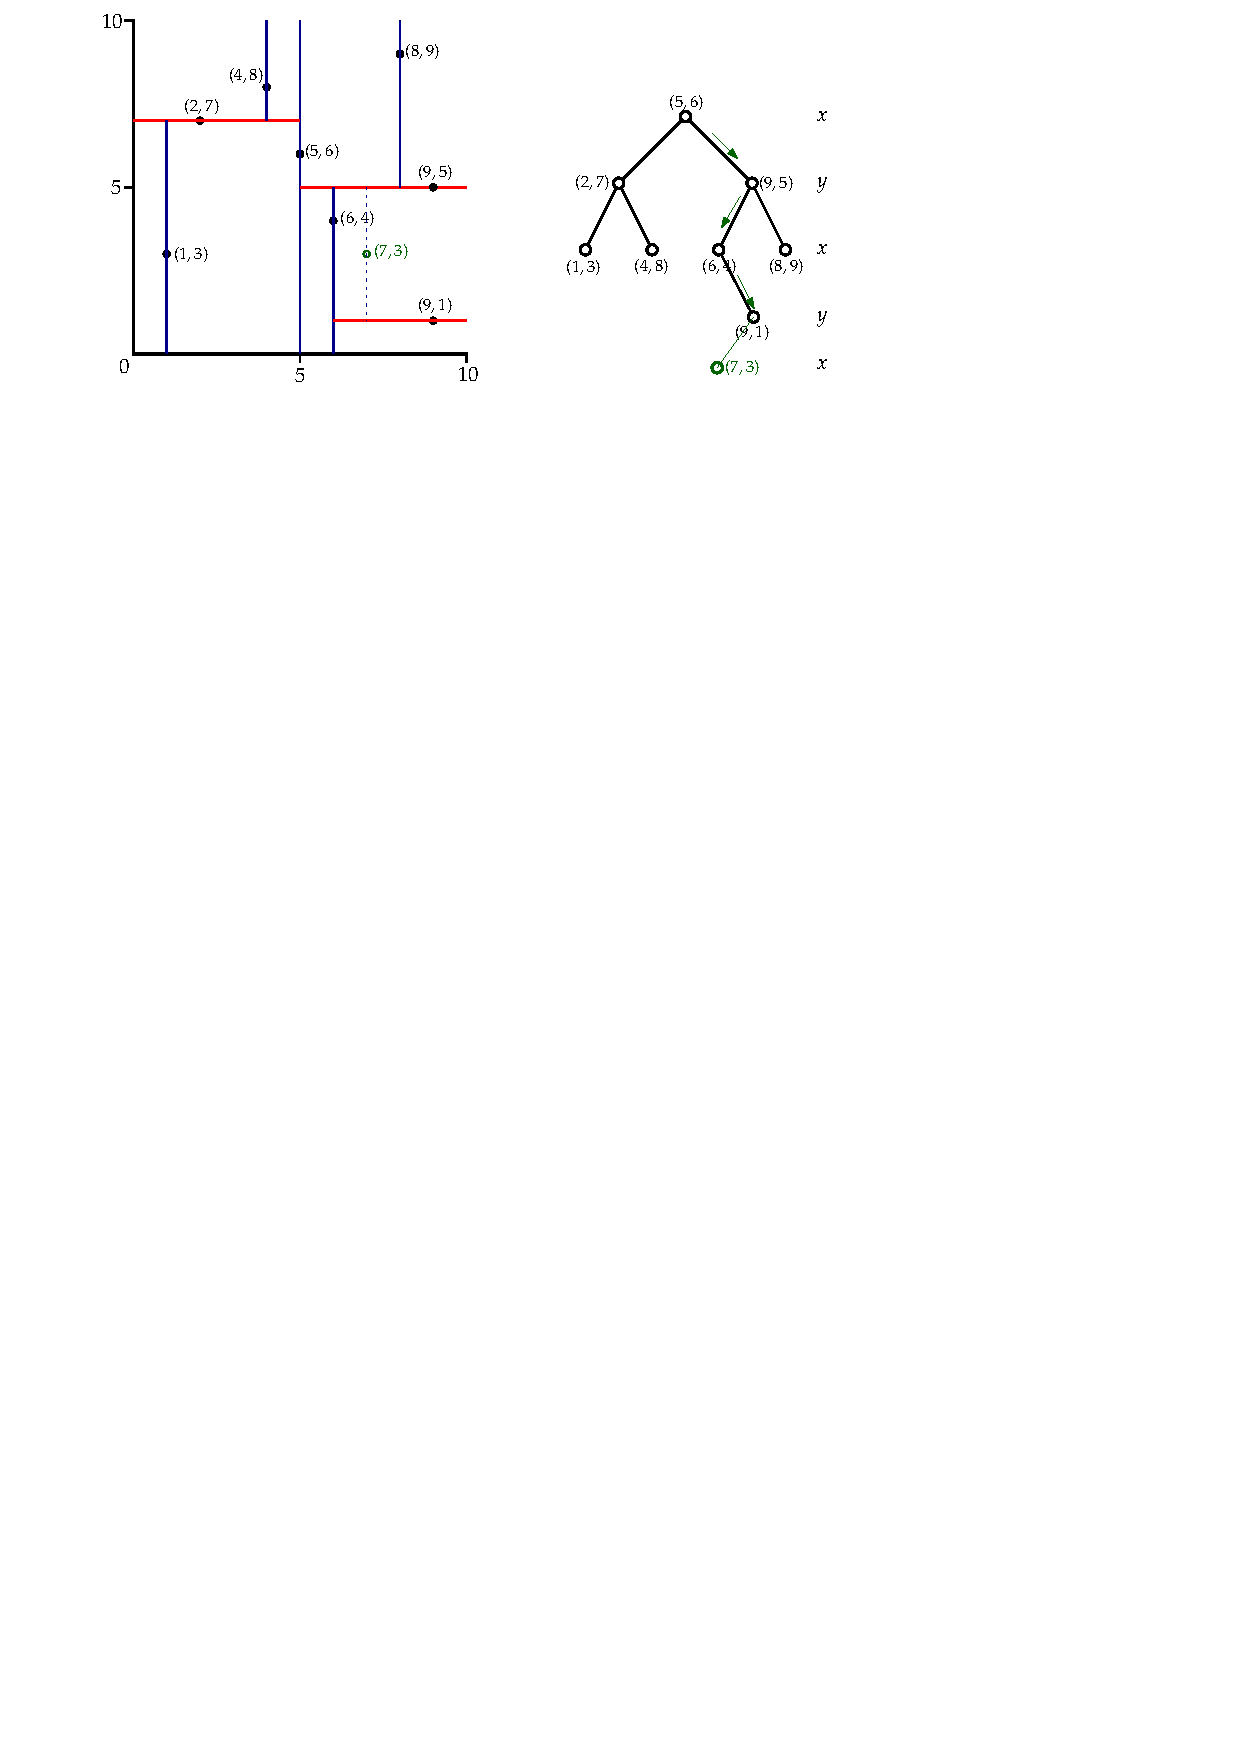
\includegraphics[width=0.9\linewidth]{figs/kdtree_insert}
  \caption{Insertion of a new point ($7,3$) in a $k$d-tree.}%
\labfig{fig:kdtree_insert}
\end{figure} 
illustrates this for one point.

Observe that this insertion renders the tree unbalanced.
Methods to balance a $k$d-tree exists but are out of scope for this course.


%%%
\paragraph{Nearest neighbour query in kd-trees.}%
\label{sec:knn}

The nearest neighbour query aims to find the point $c$ in a set $S$ that is the nearest (according to the Euclidean distance) to a query point $q$.
It can be performed brute-force (comparing distance to all points in $S$), but this is slow.
An alternative is to construct the Voronoi diagram (actually the Delaunay triangulation), and navigate in the cells; this works but is in practice not as efficient as using a $k$d-tree.

% We discuss here what a $k$d-tree, how to construct one, and how it can be used to efficiently find the nearest neighbour(s) of a query point $q$.

%

First observe that the obvious method to find the cell in the $k$d-tree containing $q$ does not work because $q$ can be far away in the tree.
\reffig{fig:kdtree_nn}a illustrates this: $c$ is ($6,4$) but is located in the right subtree of the root, while $q$ is in the left subtree.
\begin{figure*}
  \centering
  \begin{subfigure}[b]{0.6\linewidth}
    \centering
    \includegraphics[page=2,width=\textwidth]{figs/kdtree_nn.pdf}
    \caption{}
  \end{subfigure}
  \begin{subfigure}[b]{0.6\linewidth}
    \centering
    \includegraphics[page=3,width=\textwidth]{figs/kdtree_nn.pdf}
    \caption{}
  \end{subfigure}
  \begin{subfigure}[b]{0.6\linewidth}
    \centering
    \includegraphics[page=4,width=\textwidth]{figs/kdtree_nn.pdf}
    \caption{}
  \end{subfigure}
  \begin{subfigure}[b]{0.6\linewidth}
    \centering
    \includegraphics[page=5,width=\textwidth]{figs/kdtree_nn.pdf}
    \caption{}
  \end{subfigure}
\caption{Several states for the nearest neighbour query based on a $k$d-tree.}%
\labfig{fig:kdtree_nn}
\end{figure*}


%

The idea of the algorithm we are presenting here is to traverse the whole tree (in depth-first order), but use the properties of the tree to quickly eliminate large portions of the tree.
The eliminated subtrees are based on their bounding boxes.
As we traverse the tree, we must keep track of the closest point $c_{temp}$ so far visited.

% and the observation that they cannot contain any point closer

The algorithm starts at the root, stores the current closest point $c_{temp}$ as the root, and visits the nodes in the tree in the same order as for the insertion of a new point.
This order is the one that is \emph{most promising}, because we expect $c$ to be close to the insertion location (albeit this is not always the case).
At each node $n_i$ it updates $c_{temp}$ if it is closer.
For this, the Euclidean distance is used.
For the example in \reffig{fig:kdtree_nn}b, point ($5,6$) is the first $c_{temp}$, and then although ($2,7$) and ($1,3$) are visited, neither is closer and thus after that step $c_{temp} = (5,6)$.

The algorithm then recursively visits the other subtrees, and checks whether there could be any points, on the other side of the splitting hyperplane, that are closer to $q$ than $c_{temp}$.
The idea behind this step is that most of the subtrees can be eliminated by verifying whether the region of the bounding box of the subtree is closer than the current $dist(q, c_{temp})$, $dist()$ being the Euclidean distance between 2 points.
If that distance is shorter, then it is possible that one point in the subtree is closer than $c_{temp}$, and thus that subtree must be visited. 
If not, then the whole subtree can be skipped, and the algorithm continues.

\reffig{fig:kdtree_nn}c shows this idea after ($1,3$) has been visited.
$c_{temp}$ is ($5,6$), and we must decide whether the subtree right of ($2,7$) must be visited.
In this case it must not be visited because the bounding box (light blue region) is 3.0unit from $q$, and $dist(q,c_{temp})$ is around 2.07; it is thus impossible that one point inside the subtree be closer than ($5,6$).

The next step is verifying whether the subtree right of the root could contain a point closer than $c_{temp}$.
In the \reffig{fig:kdtree_nn}d, this is possible since the bounding box is only 0.5unit from $q$, and thus the subtree must be visited.

The algorithm continues until all subtrees have either been visited or eliminated.
At the end, $c$ is ($6,4$).


\paragraph{Time complexity.}
To insert a new point, and to search for a nearest neighbour, the time complexity on average is $\mathcal{O}(\log n)$.
The tree stores one node per point, thus the space complexity is $\mathcal{O}(n)$.

\paragraph{$m$-closest neighbours.}
% from Wiki
The algorithm can be extended in several ways by simple modifications. 
It can provide the $m$ nearest neighbours to a point by maintaining $m$ current closest points instead of just one. 
A branch is only eliminated when $m$ points have been found and the branch cannot have points closer than any of the $m$ current bests. 



%%%%%%%%%%%%%%%%%%%%
%
\section[Streaming paradigm]{Streaming paradigm to construct massive TINs and grids}%
\label{sec:streaming}

The incremental construction algorithm for the Delaunay triangulation, presented in \refchap{chap:dtvd}, will not work if the size of the input dataset is larger than the main memory.
Or if it works, it will be very slow.

%

To deal with massive datasets, one can also design external memory algorithms.
These basically use disks to store temporarily files that do not fit in memory, and instead of using the mechanism of the operating system, they design explicit rules for the swapping of data between the disk and the memory. 
% \citet{Agarwal05} construct massive TINs this way, and \citet{Arge06} and \citet{Agarwal08} have implemented spatial analysis functions on TINs based on that paradigm.
The main drawbacks of this approach are that the design of such algorithms is rather complex, and that for different problems different solutions have to be designed.

%

An alternative approach to dealing with massive datasets is \emph{spatial streaming},%
\index{spatial streaming}\marginnote{spatial streaming} 
which mixes ideas from external memory algorithms with different ways to keep the memory footprint very low. 
The basic idea of this paradigm is that of a \emph{streaming mesh}: a format for representing triangulations (or meshes) as a set of interleaved vertices, triangles and \emph{vertex finalization tags} that indicate when a vertex will not be used anymore.
Standard mesh formats do not use finalization and can therefore suffer if the mesh is larger than memory.
These tags allows us to keep in memory only a small part of a large dataset.

A streaming mesh basically documents the \emph{spatial coherence}%
\index{spatial coherence}\marginnote{spatial coherence} 
of a dataset, which \citet{Isenburg06} defines as: ``a correlation between the proximity in space of geometric entities and the proximity of their representations in [the file]''.
They also demonstrate that real-world point cloud datasets often have natural spatial coherence and they exploit this coherence to compute Delaunay triangulations of massive datasets (instead of reordering the points, which is expensive); this coherence is expected since LiDAR samples are often stored in the order they were collected.

The ideas behind streaming are very useful for certain \emph{local} problems (\eg\ interpolation and creation of grids), but unfortunately they cannot be used directly (or it would be extremely challenging) for \emph{global} problems such as visibility or flow modelling.

\begin{kaobox-toread}[frametitle=\faExternalLink\ To read or to watch]
  This video explains how the streaming concepts can be applied to constructing the Delaunay triangulation of massive datasets.
  You do \underline{not} need to read the full paper, which is \citet{Isenburg06}.
  \\ \\
  \url{https://youtu.be/DRCGTF2y_tM}
\end{kaobox-toread}

\begin{kaobox-toread}[frametitle=\faExternalLink\ To read or to watch]
  \fullcite{Isenburg06-1}
  \\ \\
  PDF: \url{http://dx.doi.org/10.1007/11863939_13}
  \\ \\
  The article summarises \citet{Isenburg06} (you do not need to read it), and shows how large rasters can be constructed with spatial interpolation.
\end{kaobox-toread}


%%%%%%%%%%%%%%%%%%%%
%
\section{Notes \& comments}

The description of the $k$d-tree and the nearest neighbour query is adapted from Wikipedia (\url{https://en.wikipedia.org/wiki/K-d_tree}) and the lecture notes entitled ``kd-Trees---CMSC 420'' from Carl Kingsford (available at \url{https://www.cs.cmu.edu/~ckingsf/bioinfo-lectures/kdtrees.pdf}).

\citet{Vitter01} provides an overview of external algorithms..


%%%%%%%%%%%%%%%%%%%%
%
\section{Exercises}

\begin{enumerate}
  \item \citet{Isenburg06-1} argues that real-world point cloud datasets often have natural spatial coherence. Explain why that is for lidar datasets.
  \item Given a simple point cloud stored in a CSV file (one $x,y,z$ per line), how many passes over the file does the triangulator of \citet{Isenburg06-1} make? What does each do?
  \item How to construct a $k$d-tree that is as balanced as possible?
  \item ``The ideas behind streaming are very useful for certain \emph{local} problems, but unfortunately they cannot be used directly for \emph{global} problems such as visibility or flow modelling''. Explain why that is with a concrete example.
\end{enumerate}
